% Generated by LitigCharts.PublicationFigures. Captions and provenance are sidecars.
\documentclass[10pt,tikz,border=5pt]{standalone}
\usepackage{lmodern}
\usetikzlibrary{patterns,patterns.meta}
\begin{document}
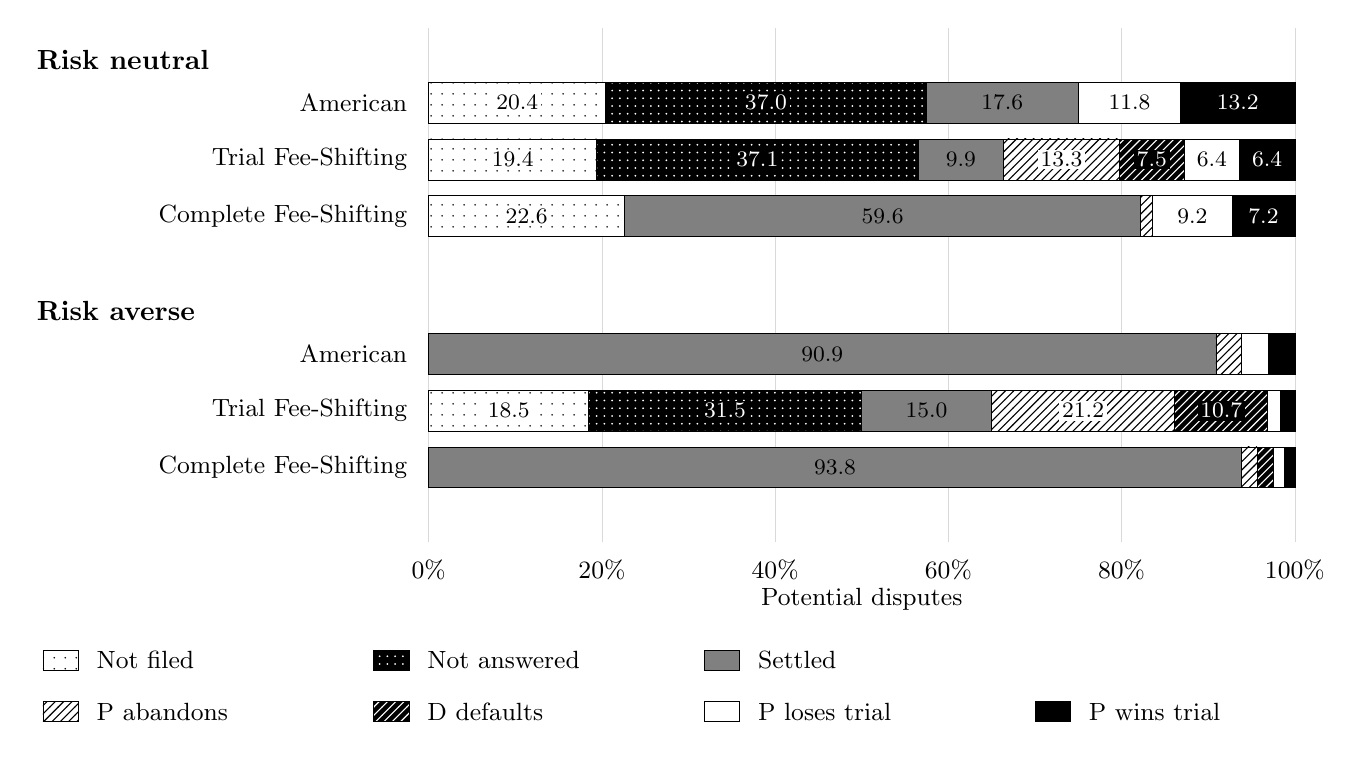
\begin{tikzpicture}[font=\small]\draw[black!15,line width=.2pt] (5.1,.65) -- (5.1,7.18);
\node[anchor=north] at (5.1,.55) {0\%};
\draw[black!15,line width=.2pt] (7.3,.65) -- (7.3,7.18);
\node[anchor=north] at (7.3,.55) {20\%};
\draw[black!15,line width=.2pt] (9.5,.65) -- (9.5,7.18);
\node[anchor=north] at (9.5,.55) {40\%};
\draw[black!15,line width=.2pt] (11.7,.65) -- (11.7,7.18);
\node[anchor=north] at (11.7,.55) {60\%};
\draw[black!15,line width=.2pt] (13.9,.65) -- (13.9,7.18);
\node[anchor=north] at (13.9,.55) {80\%};
\draw[black!15,line width=.2pt] (16.1,.65) -- (16.1,7.18);
\node[anchor=north] at (16.1,.55) {100\%};
\node[anchor=west,font=\bfseries] at (0,6.78) {\mbox{Risk} \mbox{neutral}};
\node[anchor=east] at (4.95,6.23) {American};
\path[preaction={fill=white,draw=none},pattern={Dots[distance=4pt,radius=.35pt]},pattern color=black,draw=black,line width=.25pt] (5.1,5.97) rectangle (7.347663,6.49);
\node[text=black,fill=white,font=\footnotesize,inner sep=1pt] at (6.223832,6.23) {20.4};
\path[preaction={fill=black,draw=none},pattern={Dots[distance=2.8pt,radius=.35pt]},pattern color=white,draw=black,line width=.25pt] (7.347663,5.97) rectangle (11.417553,6.49);
\node[text=white,fill=black,font=\footnotesize,inner sep=1pt] at (9.382608,6.23) {37.0};
\path[fill=black!50,draw=black,line width=.25pt] (11.417553,5.97) rectangle (13.352002,6.49);
\node[text=black,fill=none,font=\footnotesize,inner sep=1pt] at (12.384778,6.23) {17.6};
\path[fill=white,draw=black,line width=.25pt] (13.352002,5.97) rectangle (14.648693,6.49);
\node[text=black,fill=none,font=\footnotesize,inner sep=1pt] at (14.000348,6.23) {11.8};
\path[fill=black,draw=black,line width=.25pt] (14.648693,5.97) rectangle (16.1,6.49);
\node[text=white,fill=none,font=\footnotesize,inner sep=1pt] at (15.374347,6.23) {13.2};
\node[anchor=east] at (4.95,5.51) {Trial Fee-Shifting};
\path[preaction={fill=white,draw=none},pattern={Dots[distance=4pt,radius=.35pt]},pattern color=black,draw=black,line width=.25pt] (5.1,5.25) rectangle (7.233043,5.77);
\node[text=black,fill=white,font=\footnotesize,inner sep=1pt] at (6.166522,5.51) {19.4};
\path[preaction={fill=black,draw=none},pattern={Dots[distance=2.8pt,radius=.35pt]},pattern color=white,draw=black,line width=.25pt] (7.233043,5.25) rectangle (11.314967,5.77);
\node[text=white,fill=black,font=\footnotesize,inner sep=1pt] at (9.274005,5.51) {37.1};
\path[fill=black!50,draw=black,line width=.25pt] (11.314967,5.25) rectangle (12.404143,5.77);
\node[text=black,fill=none,font=\footnotesize,inner sep=1pt] at (11.859555,5.51) {9.9};
\path[preaction={fill=white,draw=none},pattern={north east lines},pattern color=black,draw=black,line width=.25pt] (12.404143,5.25) rectangle (13.870661,5.77);
\node[text=black,fill=white,font=\footnotesize,inner sep=1pt] at (13.137402,5.51) {13.3};
\path[preaction={fill=black,draw=none},pattern={north east lines},pattern color=white,draw=black,line width=.25pt] (13.870661,5.25) rectangle (14.695463,5.77);
\node[text=white,fill=black,font=\footnotesize,inner sep=1pt] at (14.283062,5.51) {7.5};
\path[fill=white,draw=black,line width=.25pt] (14.695463,5.25) rectangle (15.395414,5.77);
\node[text=black,fill=none,font=\footnotesize,inner sep=1pt] at (15.045438,5.51) {6.4};
\path[fill=black,draw=black,line width=.25pt] (15.395414,5.25) rectangle (16.100008,5.77);
\node[text=white,fill=none,font=\footnotesize,inner sep=1pt] at (15.747711,5.51) {6.4};
\node[anchor=east] at (4.95,4.79) {Complete Fee-Shifting};
\path[preaction={fill=white,draw=none},pattern={Dots[distance=4pt,radius=.35pt]},pattern color=black,draw=black,line width=.25pt] (5.1,4.53) rectangle (7.58798,5.05);
\node[text=black,fill=white,font=\footnotesize,inner sep=1pt] at (6.34399,4.79) {22.6};
\path[fill=black!50,draw=black,line width=.25pt] (7.58798,4.53) rectangle (14.142044,5.05);
\node[text=black,fill=none,font=\footnotesize,inner sep=1pt] at (10.865012,4.79) {59.6};
\path[preaction={fill=white,draw=none},pattern={north east lines},pattern color=black,draw=black,line width=.25pt] (14.142044,4.53) rectangle (14.291415,5.05);
\path[fill=white,draw=black,line width=.25pt] (14.291415,4.53) rectangle (15.304332,5.05);
\node[text=black,fill=none,font=\footnotesize,inner sep=1pt] at (14.797873,4.79) {9.2};
\path[fill=black,draw=black,line width=.25pt] (15.304332,4.53) rectangle (16.099998,5.05);
\node[text=white,fill=none,font=\footnotesize,inner sep=1pt] at (15.702165,4.79) {7.2};
\node[anchor=west,font=\bfseries] at (0,3.59) {\mbox{Risk} \mbox{averse}};
\node[anchor=east] at (4.95,3.04) {American};
\path[fill=black!50,draw=black,line width=.25pt] (5.1,2.78) rectangle (15.098208,3.3);
\node[text=black,fill=none,font=\footnotesize,inner sep=1pt] at (10.099104,3.04) {90.9};
\path[preaction={fill=white,draw=none},pattern={north east lines},pattern color=black,draw=black,line width=.25pt] (15.098208,2.78) rectangle (15.41976,3.3);
\path[fill=white,draw=black,line width=.25pt] (15.41976,2.78) rectangle (15.759876,3.3);
\path[fill=black,draw=black,line width=.25pt] (15.759876,2.78) rectangle (16.099997,3.3);
\node[anchor=east] at (4.95,2.32) {Trial Fee-Shifting};
\path[preaction={fill=white,draw=none},pattern={Dots[distance=4pt,radius=.35pt]},pattern color=black,draw=black,line width=.25pt] (5.1,2.06) rectangle (7.131623,2.58);
\node[text=black,fill=white,font=\footnotesize,inner sep=1pt] at (6.115812,2.32) {18.5};
\path[preaction={fill=black,draw=none},pattern={Dots[distance=2.8pt,radius=.35pt]},pattern color=white,draw=black,line width=.25pt] (7.131623,2.06) rectangle (10.595787,2.58);
\node[text=white,fill=black,font=\footnotesize,inner sep=1pt] at (8.863705,2.32) {31.5};
\path[fill=black!50,draw=black,line width=.25pt] (10.595787,2.06) rectangle (12.246535,2.58);
\node[text=black,fill=none,font=\footnotesize,inner sep=1pt] at (11.421161,2.32) {15.0};
\path[preaction={fill=white,draw=none},pattern={north east lines},pattern color=black,draw=black,line width=.25pt] (12.246535,2.06) rectangle (14.575477,2.58);
\node[text=black,fill=white,font=\footnotesize,inner sep=1pt] at (13.411006,2.32) {21.2};
\path[preaction={fill=black,draw=none},pattern={north east lines},pattern color=white,draw=black,line width=.25pt] (14.575477,2.06) rectangle (15.754644,2.58);
\node[text=white,fill=black,font=\footnotesize,inner sep=1pt] at (15.165061,2.32) {10.7};
\path[fill=white,draw=black,line width=.25pt] (15.754644,2.06) rectangle (15.910417,2.58);
\path[fill=black,draw=black,line width=.25pt] (15.910417,2.06) rectangle (16.099996,2.58);
\node[anchor=east] at (4.95,1.6) {Complete Fee-Shifting};
\path[fill=black!50,draw=black,line width=.25pt] (5.1,1.34) rectangle (15.41976,1.86);
\node[text=black,fill=none,font=\footnotesize,inner sep=1pt] at (10.25988,1.6) {93.8};
\path[preaction={fill=white,draw=none},pattern={north east lines},pattern color=black,draw=black,line width=.25pt] (15.41976,1.34) rectangle (15.620938,1.86);
\path[preaction={fill=black,draw=none},pattern={north east lines},pattern color=white,draw=black,line width=.25pt] (15.620938,1.34) rectangle (15.822111,1.86);
\path[fill=white,draw=black,line width=.25pt] (15.822111,1.34) rectangle (15.961051,1.86);
\path[fill=black,draw=black,line width=.25pt] (15.961051,1.34) rectangle (16.099997,1.86);
\node at (10.6,-.08) {Potential disputes};
\path[preaction={fill=white,draw=none},pattern={Dots[distance=4pt,radius=.35pt]},pattern color=black,draw=black,line width=.25pt] (0.2,-0.98) rectangle (0.65,-0.72);
\node[anchor=west] at (0.76,-0.85) {Not filed};
\path[preaction={fill=black,draw=none},pattern={Dots[distance=2.8pt,radius=.35pt]},pattern color=white,draw=black,line width=.25pt] (4.4,-0.98) rectangle (4.85,-0.72);
\node[anchor=west] at (4.96,-0.85) {Not answered};
\path[fill=black!50,draw=black,line width=.25pt] (8.6,-0.98) rectangle (9.05,-0.72);
\node[anchor=west] at (9.16,-0.85) {Settled};
\path[preaction={fill=white,draw=none},pattern={north east lines},pattern color=black,draw=black,line width=.25pt] (0.2,-1.63) rectangle (0.65,-1.37);
\node[anchor=west] at (0.76,-1.5) {P abandons};
\path[preaction={fill=black,draw=none},pattern={north east lines},pattern color=white,draw=black,line width=.25pt] (4.4,-1.63) rectangle (4.85,-1.37);
\node[anchor=west] at (4.96,-1.5) {D defaults};
\path[fill=white,draw=black,line width=.25pt] (8.6,-1.63) rectangle (9.05,-1.37);
\node[anchor=west] at (9.16,-1.5) {P loses trial};
\path[fill=black,draw=black,line width=.25pt] (12.8,-1.63) rectangle (13.25,-1.37);
\node[anchor=west] at (13.36,-1.5) {P wins trial};
\end{tikzpicture}
\end{document}
